\documentclass[conference]{IEEEtran}
\IEEEoverridecommandlockouts
% The preceding line is only needed to identify funding in the first footnote. If that is unneeded, please comment it out.
\usepackage{cite}
\usepackage{amsmath,amssymb,amsfonts}
\numberwithin{figure}{subsection}
\usepackage{algorithmic}
\usepackage{graphicx}
\usepackage{textcomp}
\usepackage{xcolor} 
\usepackage{wrapfig} 
\usepackage{enumitem}
\usepackage{algorithm}
\usepackage{algpseudocode} 
\usepackage{hyperref}
\usepackage{listings}
\usepackage{cleveref, array, booktabs, threeparttable}
\lstset{
   breaklines=true,
   basicstyle=\ttfamily
   }

\usepackage[T1]{fontenc}
\usepackage{CJKutf8}
\usepackage[english]{babel}

\graphicspath{ {./images/} }


\def\BibTeX{{\rm B\kern-.05em{\sc i\kern-.025em b}\kern-.08em
    T\kern-.1667em\lower.7ex\hbox{E}\kern-.125emX}}
\begin{document}

\title{SHOUTING PINWALL: A simple pinwall-app by team CENTRAL PERK\\}

\author{\IEEEauthorblockN{Ivo Maag}
\IEEEauthorblockA{\textit{Dept. of Computer Science} \\
\textit{Hanyang University}\\
Seoul, Republic of Korea \\
maagivo1@students.zhaw.ch}
\and

\IEEEauthorblockN{Jing Yang}
\IEEEauthorblockA{\textit{Dept. of Information Systems} \\
\textit{Hanyang University}\\
Seoul, Republic of Korea \\
alumpof@hanyang.ac.kr}
\and

\IEEEauthorblockN{Daeyoung Jung}
\IEEEauthorblockA{\textit{Dept. of Information Systems} \\
\textit{Hanyang University}\\
Seoul, Republic of Korea \\
dyjungs@gmail.com}
\and

\IEEEauthorblockN{Eonwoo Yoo}
\IEEEauthorblockA{\textit{Dept. of Information Systems} \\
\textit{Hanyang University}\\
Seoul, Republic of Korea \\
dbdjsdn123@naver.com}
}

\maketitle

\begin{abstract}
Online Bulletin Board for friends, bringing the idea of Analogue bulletin board to your mobile devices. This project is to create an Android app that uses Amazon Web Services (AWS) as a backend. It displays a pin wall where everyone can post a text. AWS will store the text in capital letters. The main purpose of this project is to learn how to use AWS and how to run software on it, how to build an Android App with backend and how to plan, document and organize a project in a team. On SHOUTING PINWALL, users can post their messages in CAPS in form of virtual post-it memo (with a character limit), on a virtual bulletin board that can only be shared with his or her friends. Through this, friends can share their stories easily. This basic app has a lot of potential for further development in case we have leftover time. For example, encryption or different media types.
 
\end{abstract}
\begin{IEEEkeywords}
SHOUTING PINWALL, Android, AWS\\
\end{IEEEkeywords}

\begin{table}[ht!] \renewcommand\arraystretch{1.25}
  \begin{threeparttable}
      \caption{Role Assignments%
      \label{tab:table1}}    %% Caption above tabular, label inside caption
      \begin{tabular}{@{}l l>{\raggedright\arraybackslash}p{3.8cm}@{}}
      \toprule
      \bfseries Role & \bfseries Name & \multicolumn{1}{l}{\bfseries Task description and etc.} \\
      \midrule
      User & Ivo & What do I need so the app is nice to use? Test the app and give feedback.\\
      
      Customer & Jing & What do we need for our company to maximize productivity? Communicate with users as well as the development team. Responsible for cost and carries risk.\\
      
      Software Developer & Daeyoung & Internal Worker. Tries to fulfill the costumers need in the code. Ideally with regular contact with Dev manager as well as costumer. Making incremental progress and shares it.\\
      
      Development manager & Eonwoo & Has an overview over budget, costumer dev. progress etc. Is in direct contact with costumer as well as dev. He has a the big picture and should detect early when things go sideways.\\
      \bottomrule
      \end{tabular}
  \end{threeparttable}
\end{table}


\newline
\section{Introduction} 
Social Media has already become a huge part of our lives and the ways we can connect to each other are so broad that we often feel things have gotten too complicated. So, we decided that we want to bring back simplicity and intuitiveness to the way we communicate. Related SW or Services: Twitter, Instagram, Facebook, etc. 
\newline

\section{Requirements}
\subsection{Functional requirements}
\begin{enumerate}
 \item As a user, I want to be able to see what other users posted.\\
 \item As a user, I want to be able post a text on the pinwall.\\
 \item As a user, I want to see an error message when sending.\\
 \item As a user, I want to see the same content, no matter which device I use.\\
 \item As a user I want to be sure my posts are saved, even if I lost my phone.\\
 \item As a user I want feedback after posting to ensure it was successful.\\
 \item As a user, when the voting phase for ‘reset’ starts I want to receive notification asking if I agree to reset the board. \\
 \item As a user, I want to receive a notification when the board is successfully cleared.\\
 \item As a user, I want to choose the color of the memo I am going to post.\\
 \item As a user, I want to delete the post I have uploaded when I want to. \\
 \item As a user, I want to set a time limit on the post I upload. When the limit expires, the post is automatically deleted. \\
 \item As a developer, I want to add further functionalities if necessary.\\
 \item As a developer, I want tests to ensure the functionality is still provided after I changed the software.\\
 \end{enumerate}
 

\subsection{General requirements}
\begin{enumerate}

 \item \textbf{Performance}: Posts should be saved and loaded within half a second after initializing the process.\\

 \item \textbf{Scalability}: The app should be able to handle up to 100 users wile staying in the set performance threshold.\\

 \item \textbf{Responsiveness}: The app should adapt to screen sizes from 4-7 inches.\\

 \item \textbf{Usability}: The functionality should be self-explanatory and not require any instruction to use it.\\

 \item \textbf{Reliability}: The app should confirm visually if a task was done successfully.\\

 \item \textbf{Security}: No security measures are planned at this point. Encryption is due to further development.\\

 \item \textbf{Availability}: The app should be available 90\% of the time, since this application is not critical.\\

 \item \textbf{Adoption to slow/no networks}: The app should display cached data if there is no connection.\\

\end{enumerate}


\section{Development environment}
\subsection{App development}
\begin{enumerate}
 \item \textbf{IDE}: Android Studio\\
    We decided to use Android Studio for development, because it's the official development tool from google and it's the only way to program native Android apps. Also all the official Documentation is made for Android Studio.\\
 
 \item \textbf{Programming language}: Kotlin / Java\\
    Kotlin is the new preferred programming language from Google. Most of the official documentation is in Kotlin. The programming language feels more modern to us than java. It compiles to Java bitecode and can even be mixed with java code in case we will need that. It gives us the opportunity to get more experience on a programming language that will most likely be very relevant in the future.\\
 
 \item \textbf{Development OS}: Ubuntu / Windows / MacOS\\
    Android Studio is officially supported for all three mentioned operating systems. We actually have all of those in use and work together cross-platform. So far this didn't cause any problems. We use MacOS 10.15, Windows 10 and Ubuntu 20.04.\\
 \end{enumerate}

\subsection{Backend}
\begin{enumerate}
 \item \textbf{AWS}: Amazon Web Services lambda
 \newline We see it as an opportunity to learn how to use a cloud environment. Our plan is to use AWS lambda for our backend. This way we don't have to worry about a physical hardware infrastructure and are still able to provide a server based service.\\
 
\end{enumerate}

\subsection{Collaboration}
\begin{enumerate}
 \item \textbf{Github}: Version Control and Collaboration of code. We use Sublime Merge as a Github desktop client.
 \newline
 \item \textbf{Kakao Talk}: Messenger to communicate among us.
 \newline
 \item \textbf{Overleaf}: It's a cloud based Latex-editor, so we can work together on the same document simultaneously.
 \newline
 \end{enumerate}

\subsection{Cost Estimation}
\textbf{Software}
\begin{enumerate}
\item Android Studio: Free
\item Kakao Talk: Free
\item Overleaf student subscription: 8 USD / Month
\item AWS: 100 credits free, which should be enough for our project.
\end{enumerate}
\textbf{Hardware}
\begin{enumerate}
\item Our personal computers: Around 5'000'000 Won. But we need them anyways for school, so we do not calculate them in.
\end{enumerate}
\textbf{Working hours}
\begin{enumerate}
\item Around five 8-hour working days per person. So around 20 working days in total. At a hypothetical 60'000 krw/hour total would be  9.6 Million Won.
\end{enumerate}
\textbf{Total}
The total would be 9.6 Million + 3 * 9k (Overleaf * 4 Months) =\textbf{ 9.627 Million Won} At this price we would probably not be very competitive in the market.
\newline


\section{Specifications}
\subsection{View Posts}
As a user, I want to be able to see what other users posted\\

To achieve this we need an Android Listview which loads the posts from the backend and displays them in chronological order.
	
\subsection{Add Posts}
As a user, I want to be able post a text on the pinwall.\\

A "+"-icon on the bottom of the screen will enable someone to add a post.
\begin{lstlisting}
    if Click '+' icon {
        moveTo Post Editing Page
            Post Editing Page() {
                1. Edit Title
                2. Edit Content (Max 140 Bytes)
                3. Select Post colour
                4. Edit View Until <date>
                5. Upload by clicking 'Upload'
            if Post Successfully Uploaded {
                alert "Posted! :D"
            }
            else
                alert "Error: Post failed :("
            }
        
        else Cancel by 'Go Back' button
    }
\end{lstlisting}

\subsection{Save Post}
As a user I want to be sure my posts are saved, even if I lost my phone.\\

To achieve this we use the amazon cloud services. Every time a user is posting, the post is automatically uploaded.

\subsection{Feedback after posting}
As a user I want feedback after posting to ensure it was successful.\\

To achieve this we simply update the view after storing it. This will give the user visual verification that it worked. If storing fails we'll need to place an error message.

\subsection{Choose Color of Memos}
As a user, I want to choose the color of the memo I am going to post.\\
\begin{lstlisting}
if User wants to choose the color of the memo
	print"What color of the memo do you prefer?"
	if color = xxx
		print memo in xxx
    print"Do you want to change the color?"
    if user click the "Yes" button{
    	repeat print"What color of the memo do you prefer?"
   		if color = xxx
    		print memo in xxx
    }
    else 
    	exit the program
\end{lstlisting}

\subsection{Delete Posts}
As a user, I want to delete the post I have uploaded when I want to. \\

If we manage to implement this feature, we need to make every post identifiable and we need a http request for the backend to delete a post.
\begin{lstlisting}
if User wants to delete the post
	DeleteThePost()
   if post successfully deleted{
		print"Deleted."
	}
	else{
		print"Error: Delete failed."
	}
\end{lstlisting}

\subsection{Add Further Functionalities}
As a developer, I want to add further functionalities if necessary.\\

We try to achieve this with a modular build and by taking care about coding standards. Code fragments that are used in multiple screens should be exported into a separate class.

\subsection{Tests}
As a developer, I want tests to ensure the functionality is still provided after I changed the software.\\

This can be done by unit tests. However, based on experience testing the UI doesn't make a lot of sence, so we should focus on functionality tests such as the following example that is thesting the validity of an e-mail address.

\begin{lstlisting}
if software changed
	TesttheFunctionality()
	if the functionality doesn't provided
		print("Something wrong with the functionality. Rewrite the code!")
	else
		exit TesttheFunctionality()
\end{lstlisting}



\subsection{Performance}
Posts  should  be  saved  and  loaded  within half a second after initializing the process.\\

Cached content should be displayed first, so if the connection is slow it doesn't wait for connection until it displays something. To display the list itself in under half a second should not be a problem.

\begin{lstlisting}
loadCachedData()
updateView()
loadFromNetwork()
updateView()
\end{lstlisting}


\subsection{Scalability}
The app should be able to handle up to 100users wile staying in the set performance threshold.\\

This should not be a problem on the frontend but maybe on the backend. Using AWS for our backend should solve this problem already since we can add resources if needed. If we get to the limit, we could assist by loading only the necessary data, for example only newly added post and not the whole list.

\begin{lstlisting}
loadNewPosts(int postNr) {
    for post in posts {
        if post.nr >= postNr {
            sendPost()
        }
    }
}
\end{lstlisting}


\subsection{Cross-device compatibility}
The  app  should  adapt  to  screen  sizes from 4-7 inches.\\

This can be achieved with constraint-layouts in Android Studio which allows to place items in relation to each other.\\


\subsection{Usability}
The  functionality  should  be  self-explanatory and not require any instruction to use it.\\

This can be achieved by naming buttons in a way that makes sense and place them in a natural way. Following Android guidelines also helps, because users are also used to the gestures from other apps. Also getting user feedback can help to achieve this.\\


\subsection{Reliability}
The  app  should  confirm  visually  if  a  task was done successfully\\

The best way to do this is probably not with pop-ups, but by displaying some kind of loading animation and updating the view after completion.

\begin{lstlisting}
postContent() --> asynchronous
displayLoading()
callback --> updateView()
\end{lstlisting}


\subsection{Security}
No security measures are planned at this point.Encryption is due to further development.\\

We decided because security is not the simplest thing to implement and would be beyond the scope of this project. But in a real-life productive application, specially if it involves personal data, proper encryption is a must.\\


\subsection{Avialability}
The  app  should  be  available  90\%  of  the time, since this application is not critical.\\

No implementation necessary. Uptime can be calculated as follows:

\begin{lstlisting}
Time of running service / Total aimed operation time.
\end{lstlisting}


\subsection{Adoption to slow/no networks}
The app should display cached data if there is no connection.\\

Also minimize network traffic can be helpful. The following article explains well how to achieve this in an android app.
\url{https://developer.android.com/training/efficient-downloads/redundant_redundant}

\begin{lstlisting}
loadContent(){
    checkIfLoadingIsNecessary()
    if yes {
        loadFromNetwork()
    } else {
        loadCache()
    }
    updateView()
}
\end{lstlisting}


\section{Screens}
\subsection{Home Screen}
The Home Screen displays our app name on the top. Under it is a Listview with all the posts loaded from the backend. On the bottom is a plus sign that can be used to create a new post.\\
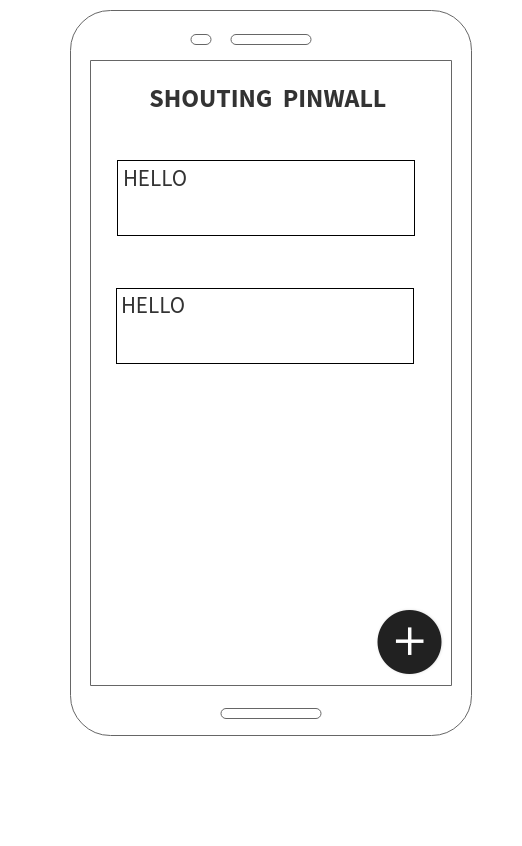
\includegraphics[width=8cm]{bibtex/images/Home_Screen.png}

\subsection{Add Post Screen}
This screen shows a button to return to the home screen alongside the app name on the top. Under it is an input field to type a post. When clicking on it, the keyboard opens and with enter-button the post can be sent.\\
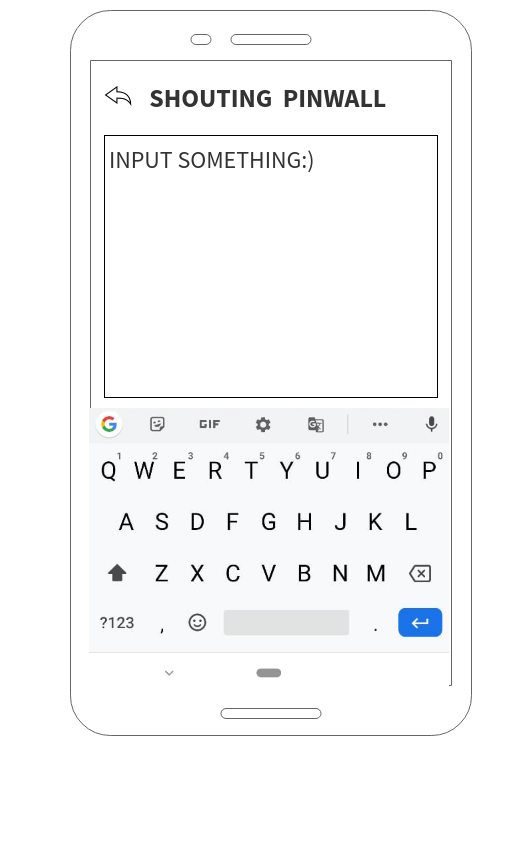
\includegraphics[width=8cm]{bibtex/images/Add_Post_Screen.png}

\subsection{Add Post Screen}
When clicking on a post on the home screen, this view opens. It shows the app name and the post in a bigger view. In the future here could be added more details such as pictures.\\
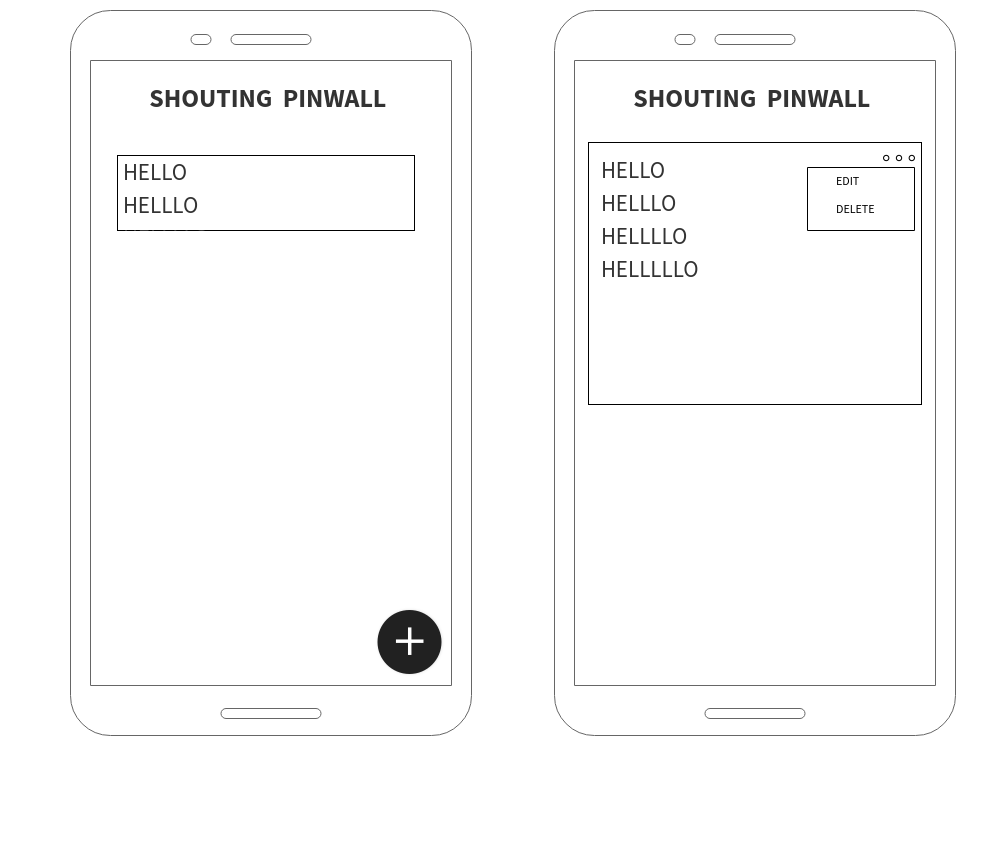
\includegraphics[width=10cm]{bibtex/images/Post_Viewing_Screen.png}


			
\end{document}